\documentclass[a4paper,12pt]{article}
\usepackage{geometry}
\usepackage{amsmath,amsfonts,amssymb}
\usepackage{graphicx}
\usepackage{subcaption}
\usepackage{caption}
\usepackage{booktabs}
\usepackage{hyperref}
\usepackage{enumitem}
\setlist[itemize]{label=$\bullet$}
\setlength{\headheight}{15pt}
\usepackage{xcolor}
\usepackage{titling}
\usepackage{fancyhdr}
\usepackage{parskip}
\usepackage{listings}
\usepackage{float}

% Custom colors
\definecolor{titleblue}{RGB}{0,102,204}
\definecolor{headingblue}{RGB}{0,51,102}

% Code listing style
\lstset{
    language=Python,
    basicstyle=\ttfamily\footnotesize,
    keywordstyle=\color{blue}\bfseries,
    stringstyle=\color{purple},
    commentstyle=\color{gray}\itshape,
    numberstyle=\tiny,
    numbers=left,
    stepnumber=1,
    numbersep=5pt,
    showspaces=false,
    showstringspaces=false,
    frame=single,
    breaklines=true,
    breakatwhitespace=true,
    tabsize=4
}

% Page layout
\geometry{top=2.5cm,bottom=2.5cm,left=2.5cm,right=2.5cm}
\setlength{\parindent}{0pt}
\setlength{\parskip}{0.8em}

% Header and footer
\pagestyle{fancy}
\fancyhf{}
\fancyhead[L]{\textbf{INS3155 - Computer Vision Midterm Report}}
\fancyhead[R]{Midterm Project Report}
\fancyfoot[C]{\thepage}

% Title customization
\pretitle{\centering\LARGE\bfseries}
\posttitle{\vspace{0.4cm}}
\preauthor{\centering}
\postauthor{}
\predate{\centering}
\postdate{}

\begin{document}

\title{\textcolor{titleblue}{Midterm Project Report:\\Traditional Image Processing for Filtering, 3D Reconstruction, and Image Stitching}}

\author{\parbox{0.7\linewidth}{\centering
Name: Student Full Name\\
Student ID: StudentID\\
Course: INS3155 -- Computer Vision}}

\date{October 2026}

\maketitle

\begin{abstract}
This report presents a complete implementation and quantitative/qualitative evaluation of classical computer vision methods across three core tasks using a custom architectural reference photograph (\texttt{IMG\_0891.jpg}) for Parts A and C and the Middlebury Teddy stereo pair for Part B. In \textbf{Part A}, we synthesize Gaussian ($\sigma=25$) and Salt-and-Pepper ($8\%$) noise and evaluate four spatial filters (Mean, Gaussian, Median, and Laplacian Sharpening) across $3\times 3$, $5\times 5$, and $7\times 7$ kernels. Experimental results show that the $3\times 3$ Gaussian filter achieves the highest PSNR ($24.77\text{ dB}$) on Gaussian noise, whereas the $3\times 3$ Median filter dominates on impulsive Salt-and-Pepper noise ($26.80\text{ dB}$ PSNR, $0.9285$ SSIM). In \textbf{Part B}, we use the Middlebury Teddy stereo pair with ground-truth disparity, estimate the Fundamental Matrix via SIFT and RANSAC (mean epipolar error $0.2389\text{ px}$ across $315$ inliers), and compare Block Matching (BM) against Semi-Global Block Matching (SGBM) for dense disparity and 3D point cloud reconstruction. SGBM ($b=3$) raises valid disparity coverage from about $70\%$ to $81.12\%$ and achieves the lowest bad-pixel rate ($3.43\%$ of non-occluded pixels with error $>2$ px). In \textbf{Part C}, we construct an end-to-end 4-view panoramic stitching pipeline comparing SIFT, ORB, and AKAZE detectors with distance-transform feather blending, achieving sub-pixel reprojection accuracy ($0.192\text{ px}$--$0.256\text{ px}$ RMSE).
\end{abstract}

\section{Introduction}
Traditional image processing and geometric computer vision form the mathematical backbone of modern visual perception systems. Unlike black-box deep neural networks, classical operators offer analytical interpretability, deterministic runtime on standard CPUs, and zero dependency on large-scale training datasets.

This project investigates three fundamental problems, using a high-contrast architectural wall image featuring intricate geometric fretwork and ornamental reliefs for Parts A and C, and the Middlebury Teddy stereo benchmark for Part B:
\begin{itemize}
    \item \textbf{Part A (Image Filtering \& Enhancement):} Mitigating thermal sensor noise (Gaussian) and transmission bit errors (Salt-and-Pepper) while preserving sharp geometric boundaries and enhancing high-frequency details via second-order Laplacian derivatives.
    \item \textbf{Part B (3D Stereo Reconstruction):} Recovering epipolar geometry via the Fundamental Matrix $\mathbf{F}$, computing dense disparity maps via local Block Matching (BM) and Semi-Global Block Matching (SGBM), and triangulating a 3D point cloud on the Middlebury Teddy stereo pair, whose ground-truth disparity enables accuracy evaluation.
    \item \textbf{Part C (Multi-View Image Stitching):} Extracting and matching local invariant features across four overlapping perspective views, estimating planar homographies via RANSAC, and seamlessly blending the warped views into a unified panorama.
\end{itemize}

\section{Part A: Image Filtering}
\subsection{Methodology}
Given a clean grayscale image $I(x,y) \in [0,255]$ of size $640\times 480$, we synthesize two noisy observations $\tilde{I}(x,y)$:
\begin{enumerate}
    \item \textbf{Additive White Gaussian Noise (AWGN):} $\tilde{I}(x,y) = \text{clip}(I(x,y) + \eta(x,y), 0, 255)$ with $\eta \sim \mathcal{N}(0, \sigma_n^2)$, $\sigma_n = 25$.
    \item \textbf{Salt-and-Pepper Noise:} Each pixel is independently set to $255$ with probability $p_s = 0.04$ or $0$ with probability $p_p = 0.04$ (total corruption rate $8\%$).
\end{enumerate}
We evaluate four spatial filters across kernel sizes $k \in \{3, 5, 7\}$ (half-width $a = (k-1)/2$):
\begin{itemize}
    \item \textbf{Mean (Box) Filter:} Uniform spatial averaging $\hat{I}(x,y) = \frac{1}{k^2}\sum_{i=-a}^{a}\sum_{j=-a}^{a}\tilde{I}(x+i,y+j)$.
    \item \textbf{Gaussian Filter:} Weighted convolution with $G_\sigma(i,j) = \frac{1}{2\pi\sigma^2}\exp\left(-\frac{i^2+j^2}{2\sigma^2}\right)$ using $\sigma \in \{0.8, 1.2, 1.6\}$ for $k \in \{3,5,7\}$.
    \item \textbf{Median Filter:} Non-linear order-statistic operator $\hat{I}(x,y) = \text{median}_{(i,j)\in W_k}\{\tilde{I}(x+i,y+j)\}$.
    \item \textbf{Laplacian Sharpening:} Applied to the denoised image $\hat{I}$ to restore high-frequency step edges:
    $$\hat{I}_{\text{sharp}}(x,y) = \text{clip}\left(\hat{I}(x,y) - \alpha \nabla^2 \hat{I}(x,y),\, 0,\, 255\right), \quad \nabla^2 \hat{I} = \frac{\partial^2 \hat{I}}{\partial x^2} + \frac{\partial^2 \hat{I}}{\partial y^2}$$
\end{itemize}

\subsection{Implementation and Results}
Figure \ref{fig:part_a_grids} displays the visual comparison grids for both Gaussian and Salt-and-Pepper noise across all four filters and kernel sizes ($3\times 3$, $5\times 5$, $7\times 7$).

\begin{figure}[H]
    \centering
    \begin{subfigure}{\textwidth}
        \centering
        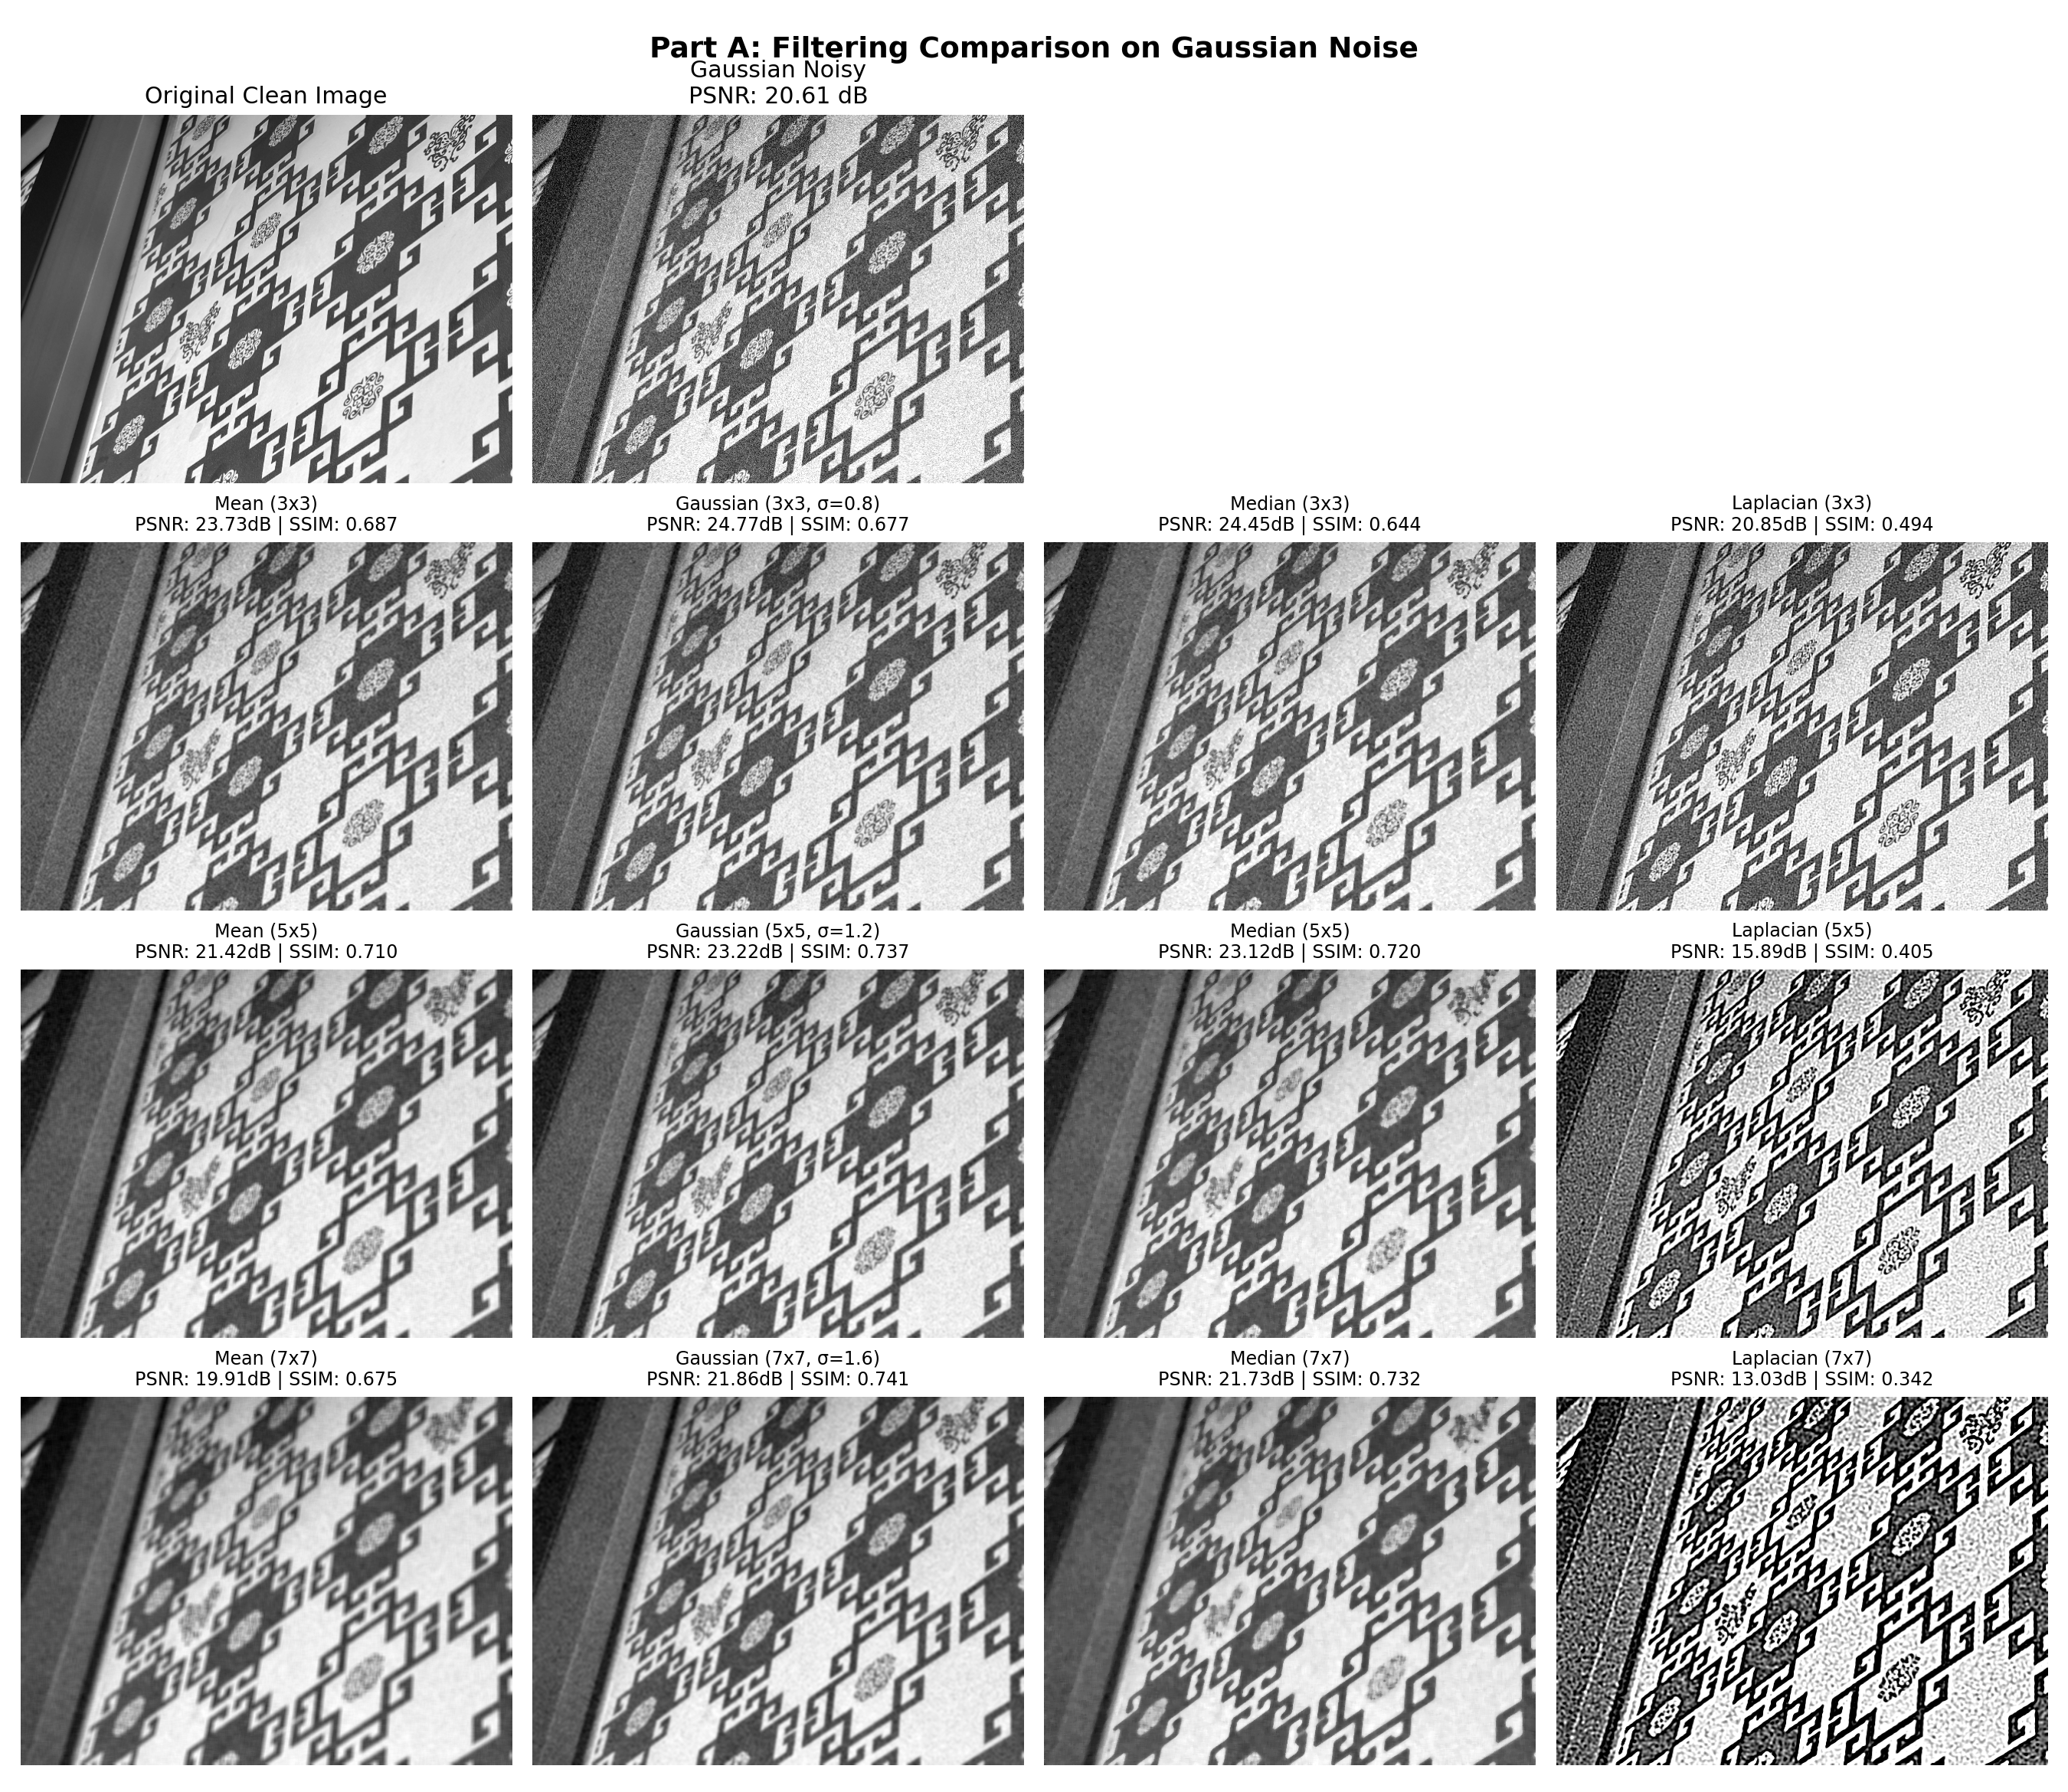
\includegraphics[width=0.92\textwidth]{figures/grid_Gaussian.png}
        \caption{Filtering and sharpening results on Gaussian noise ($\sigma=25$).}
    \end{subfigure}
    \vspace{0.3cm}
    \begin{subfigure}{\textwidth}
        \centering
        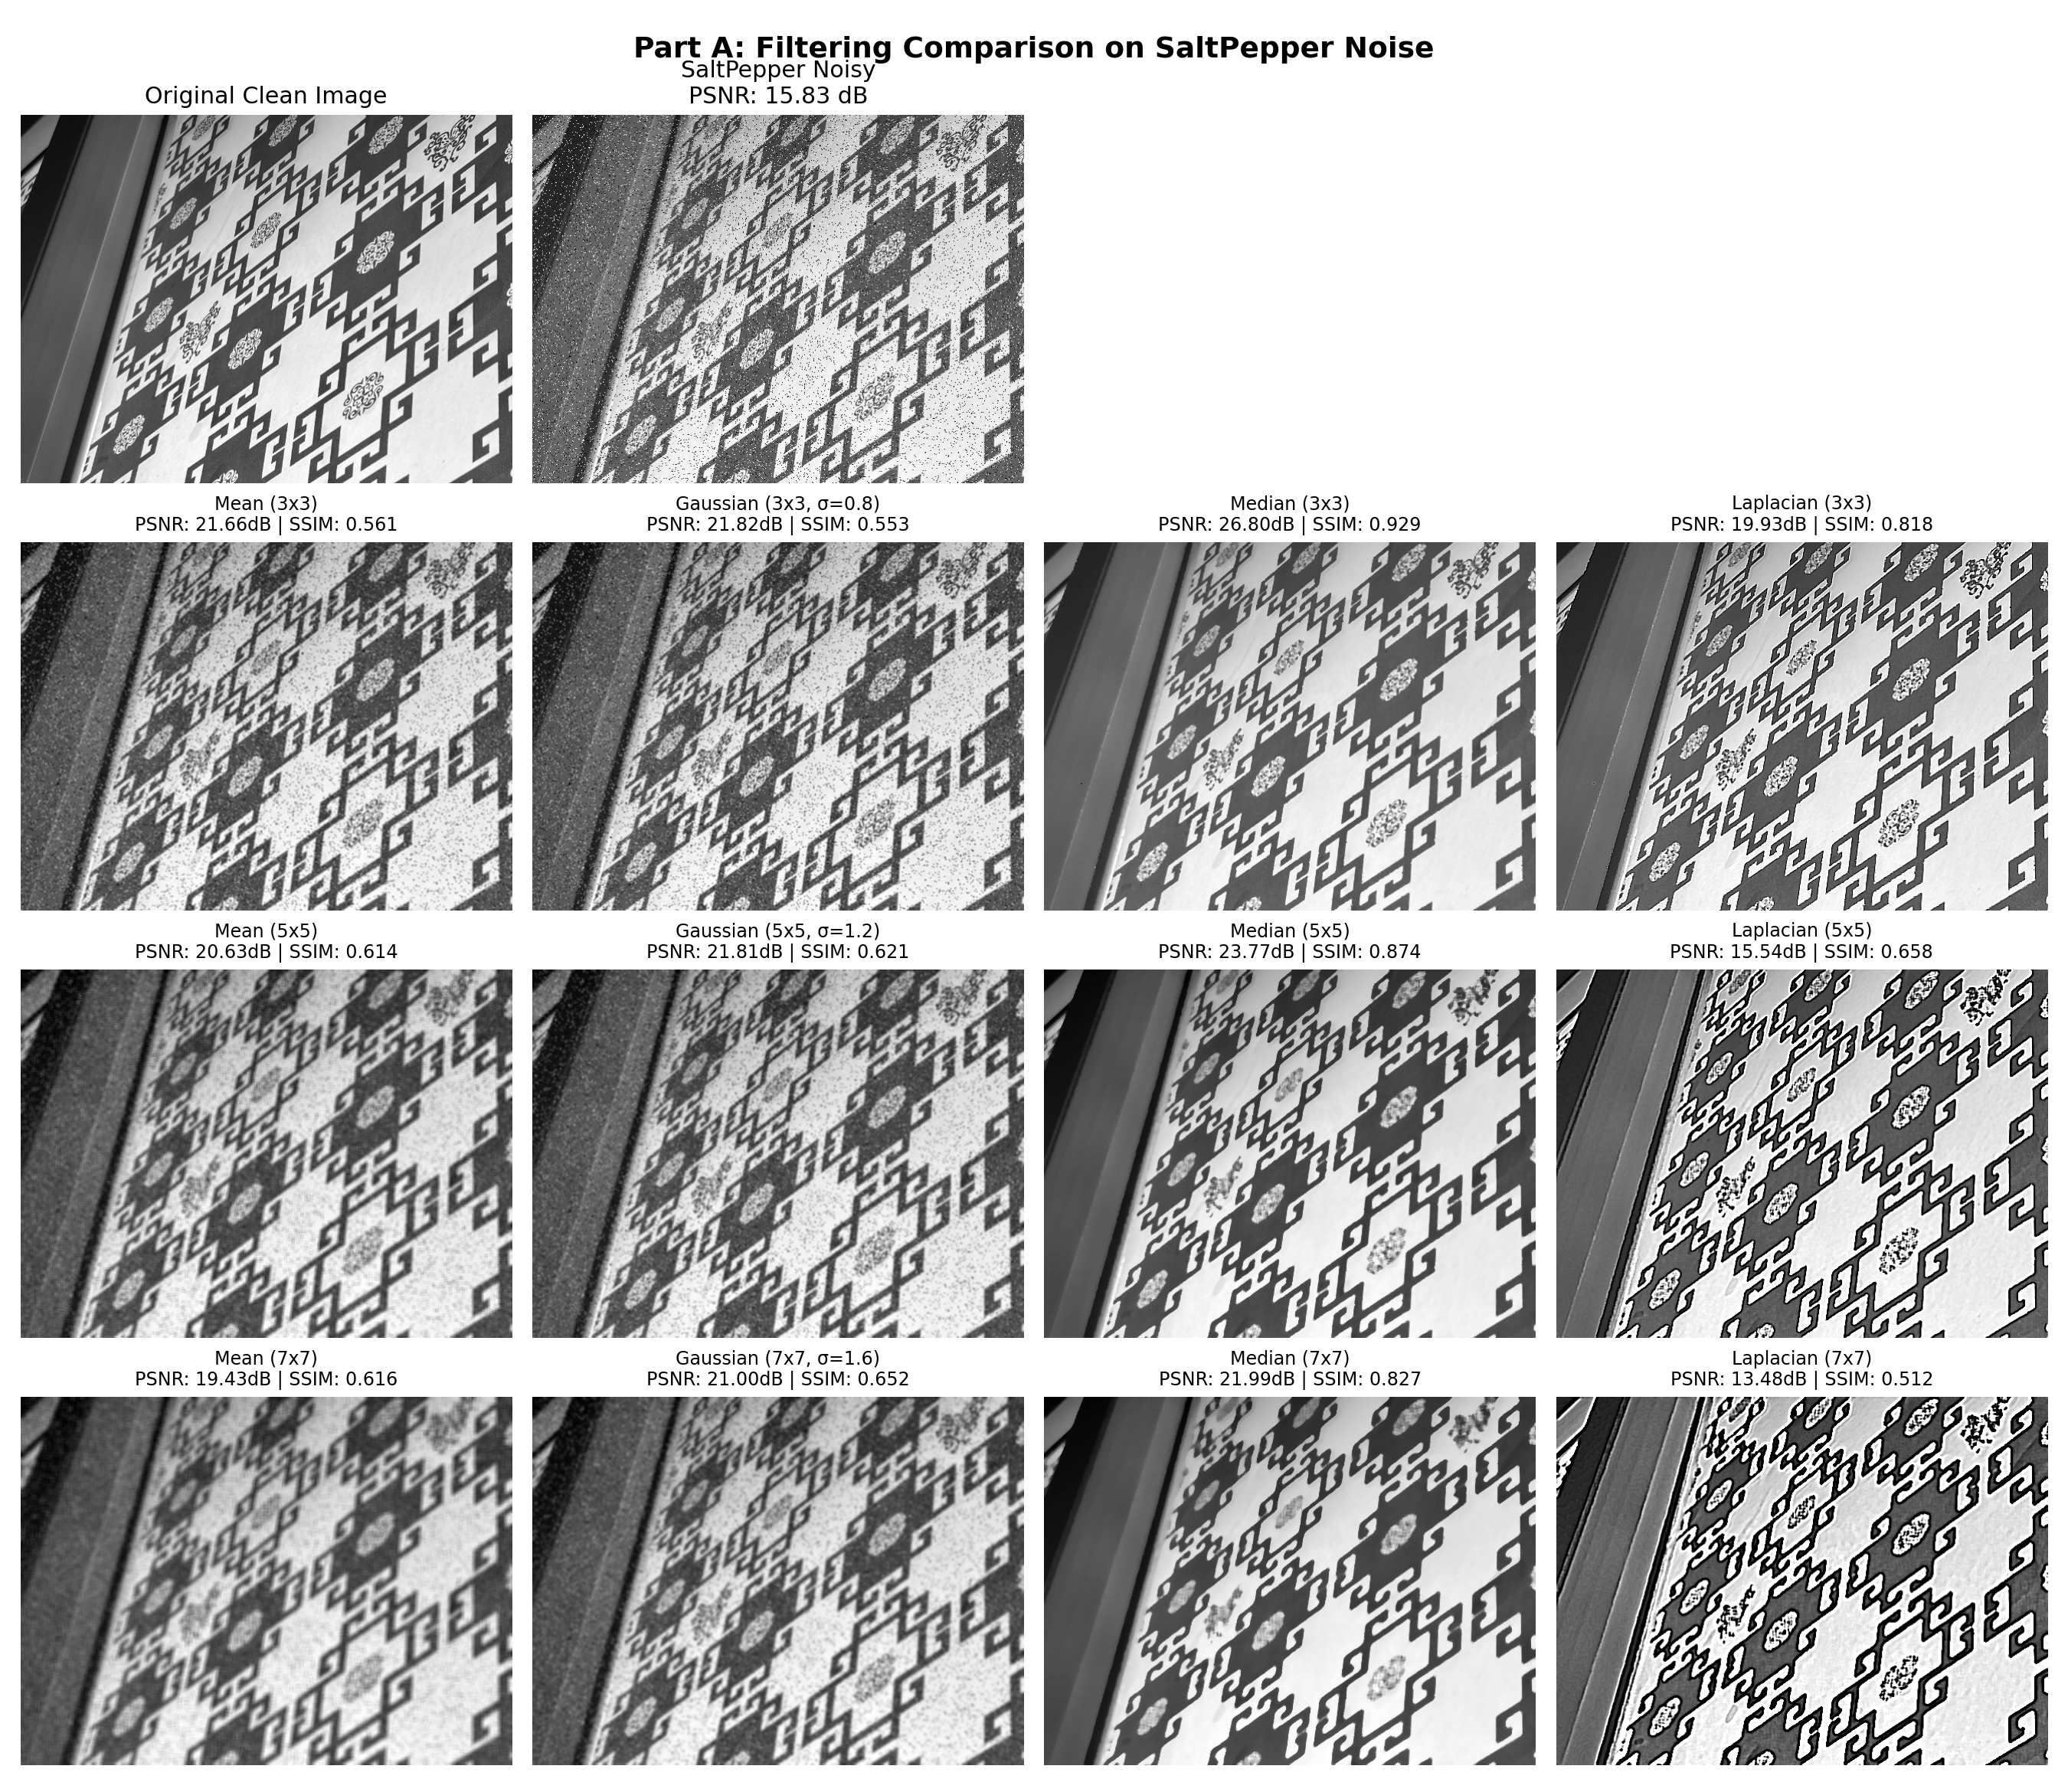
\includegraphics[width=0.92\textwidth]{figures/grid_SaltPepper.png}
        \caption{Filtering and sharpening results on Salt-and-Pepper noise ($p_s=p_p=0.04$).}
    \end{subfigure}
    \caption{Part A visual grids comparing Original, Noisy, Mean, Gaussian, Median, and Laplacian Sharpening across $3\times 3$, $5\times 5$, and $7\times 7$ kernels.}
    \label{fig:part_a_grids}
\end{figure}

\subsection{Comparative Analysis}
Table \ref{tab:part_a} reports the quantitative performance in terms of MSE, PSNR (dB), SSIM, and runtime (ms).

\begin{table}[H]
\centering
\caption{Quantitative evaluation of spatial filters on Gaussian and Salt-and-Pepper noise.}
\label{tab:part_a}
\footnotesize
\begin{tabular}{llccccc}
\toprule
\textbf{Noise Type} & \textbf{Filter \& Parameter} & \textbf{Kernel} & \textbf{MSE} $\downarrow$ & \textbf{PSNR (dB)} $\uparrow$ & \textbf{SSIM} $\uparrow$ & \textbf{Time (ms)} $\downarrow$ \\
\midrule
Gaussian ($\sigma=25$) & Mean Filter & $3\times 3$ & 275.44 & 23.73 & 0.6868 & 0.863 \\
Gaussian ($\sigma=25$) & Gaussian ($\sigma=0.8$) & $3\times 3$ & \textbf{216.86} & \textbf{24.77} & 0.6766 & 0.595 \\
Gaussian ($\sigma=25$) & Median Filter & $3\times 3$ & 233.64 & 24.45 & 0.6438 & 1.302 \\
Gaussian ($\sigma=25$) & Laplacian Sharp & $3\times 3$ & 534.29 & 20.85 & 0.4944 & 9.929 \\
Gaussian ($\sigma=25$) & Mean Filter & $5\times 5$ & 468.50 & 21.42 & 0.7102 & \textbf{0.353} \\
Gaussian ($\sigma=25$) & Gaussian ($\sigma=1.2$) & $5\times 5$ & 309.89 & 23.22 & 0.7370 & 0.611 \\
Gaussian ($\sigma=25$) & Median Filter & $5\times 5$ & 317.04 & 23.12 & 0.7200 & 5.310 \\
Gaussian ($\sigma=25$) & Gaussian ($\sigma=1.6$) & $7\times 7$ & 423.32 & 21.86 & \textbf{0.7409} & 0.361 \\
Gaussian ($\sigma=25$) & Median Filter & $7\times 7$ & 436.39 & 21.73 & 0.7323 & 18.351 \\
\midrule
Salt \& Pepper ($8\%$) & Mean Filter & $3\times 3$ & 443.24 & 21.66 & 0.5606 & 0.463 \\
Salt \& Pepper ($8\%$) & Gaussian ($\sigma=0.8$) & $3\times 3$ & 427.28 & 21.82 & 0.5530 & \textbf{0.314} \\
Salt \& Pepper ($8\%$) & Median Filter & $3\times 3$ & \textbf{135.81} & \textbf{26.80} & \textbf{0.9285} & 0.747 \\
Salt \& Pepper ($8\%$) & Laplacian Sharp & $3\times 3$ & 660.52 & 19.93 & 0.8182 & 2.504 \\
Salt \& Pepper ($8\%$) & Mean Filter & $5\times 5$ & 562.87 & 20.63 & 0.6139 & 0.326 \\
Salt \& Pepper ($8\%$) & Gaussian ($\sigma=1.2$) & $5\times 5$ & 428.99 & 21.81 & 0.6207 & 0.378 \\
Salt \& Pepper ($8\%$) & Median Filter & $5\times 5$ & 272.66 & 23.77 & 0.8742 & 3.809 \\
Salt \& Pepper ($8\%$) & Median Filter & $7\times 7$ & 410.97 & 21.99 & 0.8274 & 18.609 \\
\bottomrule
\end{tabular}
\end{table}

\textbf{Qualitative Observations:}
\begin{itemize}
    \item \textbf{Noise Removal vs. Edge Preservation:} Because the reference image contains high-contrast geometric fretwork and intricate floral motifs, expanding the kernel from $3\times 3$ to $7\times 7$ causes severe \textit{over-smoothing} of thin lines, increasing MSE on clean edges. Consequently, $3\times 3$ Gaussian filtering achieves the best PSNR ($24.77\text{ dB}$) under AWGN, while $7\times 7$ Gaussian achieves the highest structural similarity ($\text{SSIM}=0.7409$) by smoothing homogeneous wall regions.
    \item \textbf{Impulsive Noise Robustness:} Linear filters (Mean and Gaussian) fail on Salt-and-Pepper noise because extreme $0/255$ impulses are averaged into gray speckles. The non-linear \textbf{Median ($3\times 3$)} filter completely eliminates impulse noise while keeping sharp fretwork corners intact ($\text{PSNR}=26.80\text{ dB}$, $\text{SSIM}=0.9285$).
    \item \textbf{Halo and Ringing Artifacts:} Laplacian sharpening visibly crisps the architectural borders, but larger Laplacian kernels ($5\times 5, 7\times 7$) amplify residual high-frequency noise and produce overshoot \textit{halo/ringing artifacts} along step edges.
\end{itemize}

\section{Part B: 3D Reconstruction}
\subsection{Dataset}
Part B uses the \textbf{Middlebury 2003 Teddy} stereo pair \cite{middlebury}: \texttt{im2.png} (left view $I_L$) and \texttt{im6.png} (right view $I_R$), both $450\times 375$ pixels and already rectified. The dataset also provides dense ground-truth disparity maps for both views (\texttt{disp2.png}, \texttt{disp6.png}) stored as $4\times$ the true disparity, with $0$ marking unknown pixels. After rescaling, the ground-truth disparity of the left view ranges from $12.50$ to $52.75$ px. A pixel of the left view is labelled \emph{non-occluded} when its ground-truth disparity is consistent with the right ground truth: $|d_R(x - d_L(x,y), y) - d_L(x,y)| \le 1$ px. This mask covers $87.26\%$ of the image and is used for all accuracy metrics.

\subsection{Methodology}
SIFT keypoints of $(I_L, I_R)$ are matched using 2-NN search with Lowe's ratio test ($0.75$). The Fundamental Matrix $\mathbf{F} \in \mathbb{R}^{3\times 3}$ is estimated via RANSAC (threshold $1.0$ px, confidence $0.999$) to enforce the epipolar constraint $\mathbf{x}_R^\top \mathbf{F} \mathbf{x}_L = 0$. Two geometric errors are reported over the $N$ inliers, the symmetric point-to-epipolar-line distance and the first-order Sampson distance:
$$E_{\text{epi}} = \frac{1}{2N}\sum_{i=1}^{N}\left(\frac{|\mathbf{l}_{R,i}^\top \mathbf{x}_{R,i}|}{\sqrt{l_{R,i,1}^2 + l_{R,i,2}^2}} + \frac{|\mathbf{l}_{L,i}^\top \mathbf{x}_{L,i}|}{\sqrt{l_{L,i,1}^2 + l_{L,i,2}^2}}\right)$$
$$E_{\text{samp}} = \frac{1}{N}\sum_{i=1}^{N}\frac{|\mathbf{x}_{R,i}^\top \mathbf{F}\mathbf{x}_{L,i}|}{\sqrt{(\mathbf{F}\mathbf{x}_{L,i})_1^2 + (\mathbf{F}\mathbf{x}_{L,i})_2^2 + (\mathbf{F}^\top\mathbf{x}_{R,i})_1^2 + (\mathbf{F}^\top\mathbf{x}_{R,i})_2^2}}$$
Dense disparity maps $d(x,y) = x_L - x_R$ are then computed with local \textbf{Block Matching (BM)} (Sum of Absolute Differences over a $b\times b$ window on grayscale images) and \textbf{Semi-Global Block Matching (SGBM)} \cite{hirschmuller} (color matching cost aggregated along multiple 1D paths with smoothness penalties $P_1 = 24b^2$ and $P_2 = 96b^2$). Both methods use uniqueness ratio $10$ and speckle filtering (window $100$, range $2$). Accuracy is measured on valid estimates inside the non-occluded mask $\Omega$:
$$\text{RMSE} = \sqrt{\frac{1}{|\Omega|}\sum_{(x,y)\in\Omega}\left(d(x,y) - d_{\text{GT}}(x,y)\right)^2}, \qquad \text{Bad}_{\tau} = \frac{100}{|\Omega|}\sum_{(x,y)\in\Omega}\left[\,|d(x,y) - d_{\text{GT}}(x,y)| > \tau\,\right], \; \tau\in\{1, 2\}$$
Runtime is the median of five runs. Finally, 3D points are triangulated with $\mathbf{Q}$ as $Z = fB/d$, $X = (x - c_x)Z/f$, $Y = (y - c_y)Z/f$. Teddy is distributed without calibration, so we assume $f = 450$ px and $B = 0.16$ m; the recovered shape is correct up to this global scale.

\subsection{Implementation and Results}
SIFT detects $706$ and $729$ keypoints in the left and right views. Of the $337$ ratio-test matches, $315$ are RANSAC inliers ($93.47\%$), giving a mean epipolar error of $0.2389$ px and a mean Sampson error of $0.1689$ px. Because Teddy is rectified, the epipolar lines in Figure \ref{fig:epipolar} are horizontal and the inliers differ by only $0.17$ px vertically on average. Figure \ref{fig:disparity} compares the colorized disparity maps of BM and SGBM with the ground truth, Figure \ref{fig:errormaps} localizes the errors of the best BM and SGBM settings, and Figure \ref{fig:pointcloud} shows the reconstructed point cloud.

\begin{figure}[H]
    \centering
    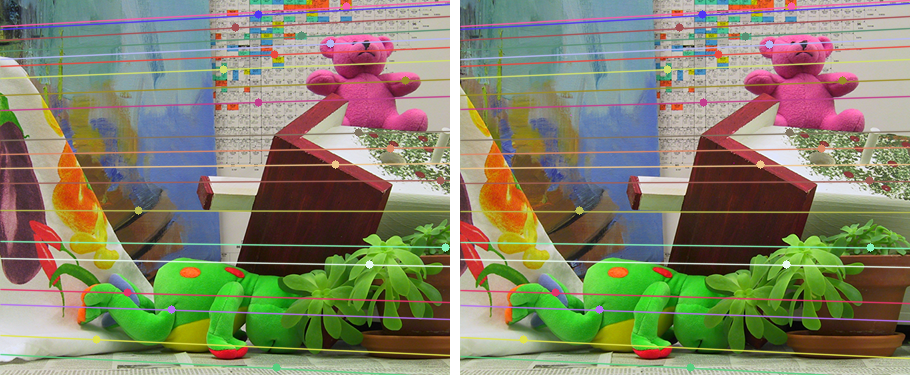
\includegraphics[width=0.95\textwidth]{figures/epipolar_lines.png}
    \caption{Part B: Epipolar lines on the Teddy left (\texttt{im2}) and right (\texttt{im6}) views using $\mathbf{F}$ estimated via RANSAC.}
    \label{fig:epipolar}
\end{figure}

\begin{figure}[H]
    \centering
    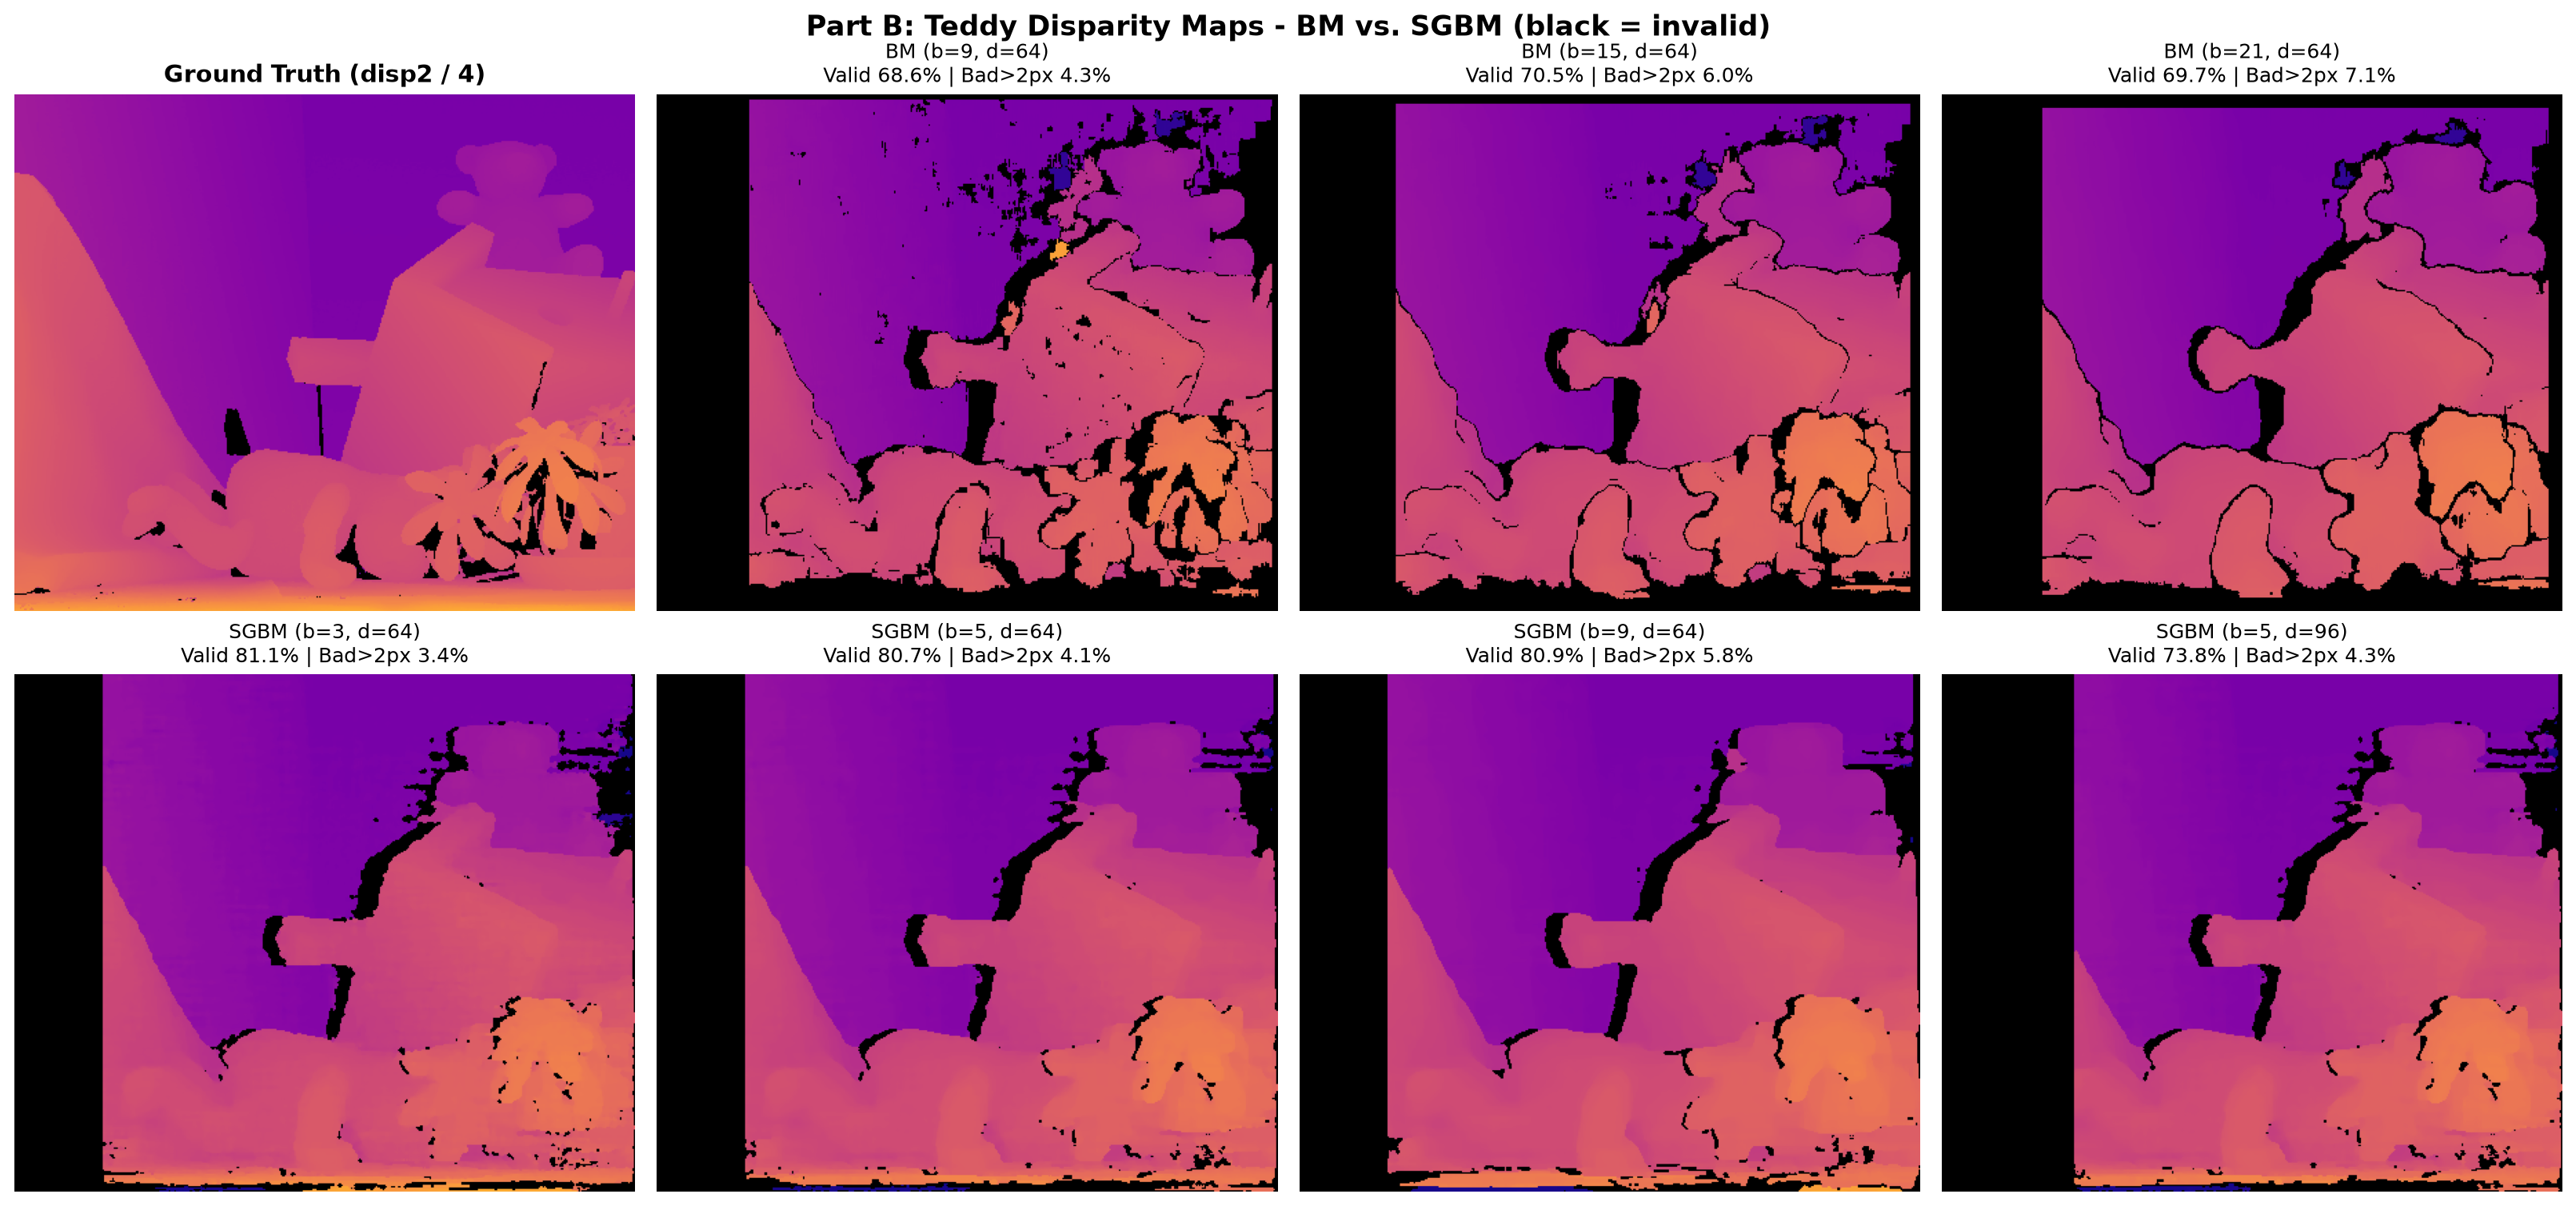
\includegraphics[width=\textwidth]{figures/disparity_comparison.png}
    \caption{Part B: Ground-truth disparity and dense disparity maps for BM ($b \in \{9, 15, 21\}$) and SGBM ($b \in \{3, 5, 9\}$, $d \in \{64, 96\}$). Black pixels are invalid.}
    \label{fig:disparity}
\end{figure}

\begin{figure}[H]
    \centering
    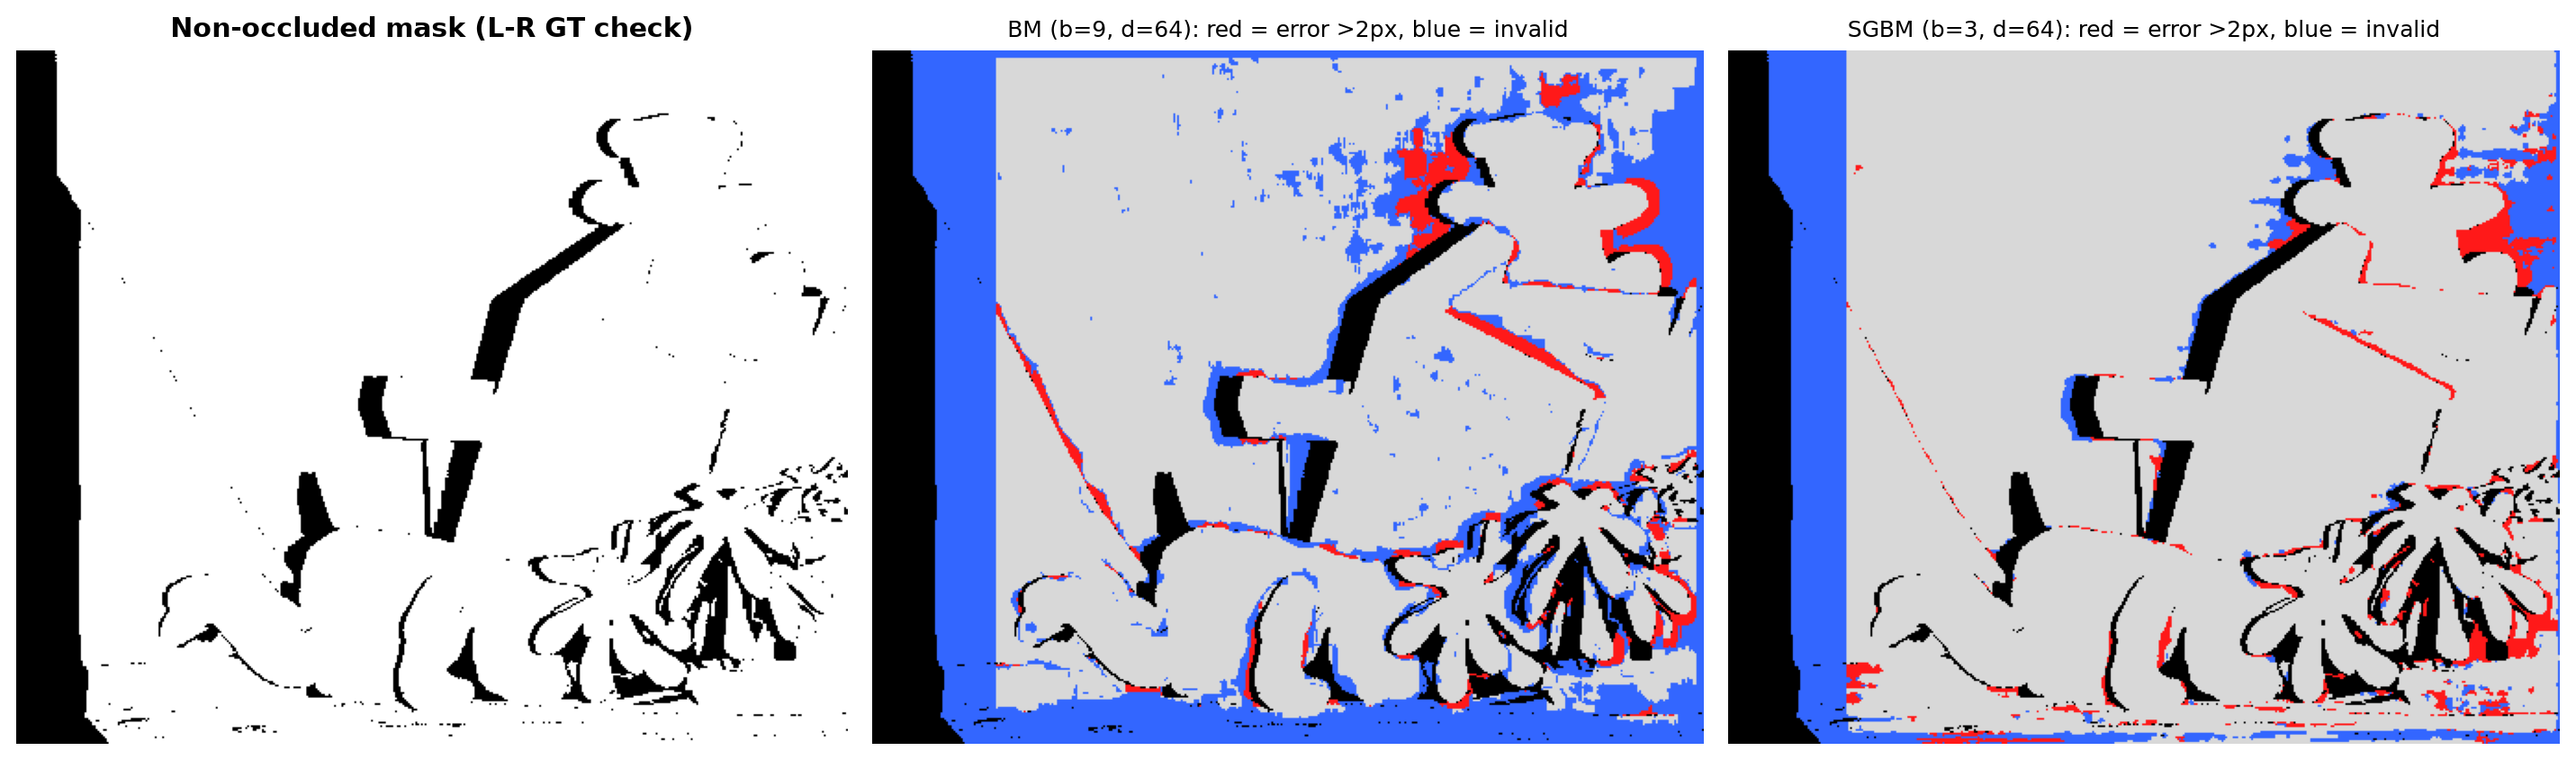
\includegraphics[width=\textwidth]{figures/disparity_error_maps.png}
    \caption{Part B: Non-occluded evaluation mask and error maps of the best BM and SGBM settings (red: error $>2$ px, blue: invalid estimate, black: occluded or unknown).}
    \label{fig:errormaps}
\end{figure}

\begin{figure}[H]
    \centering
    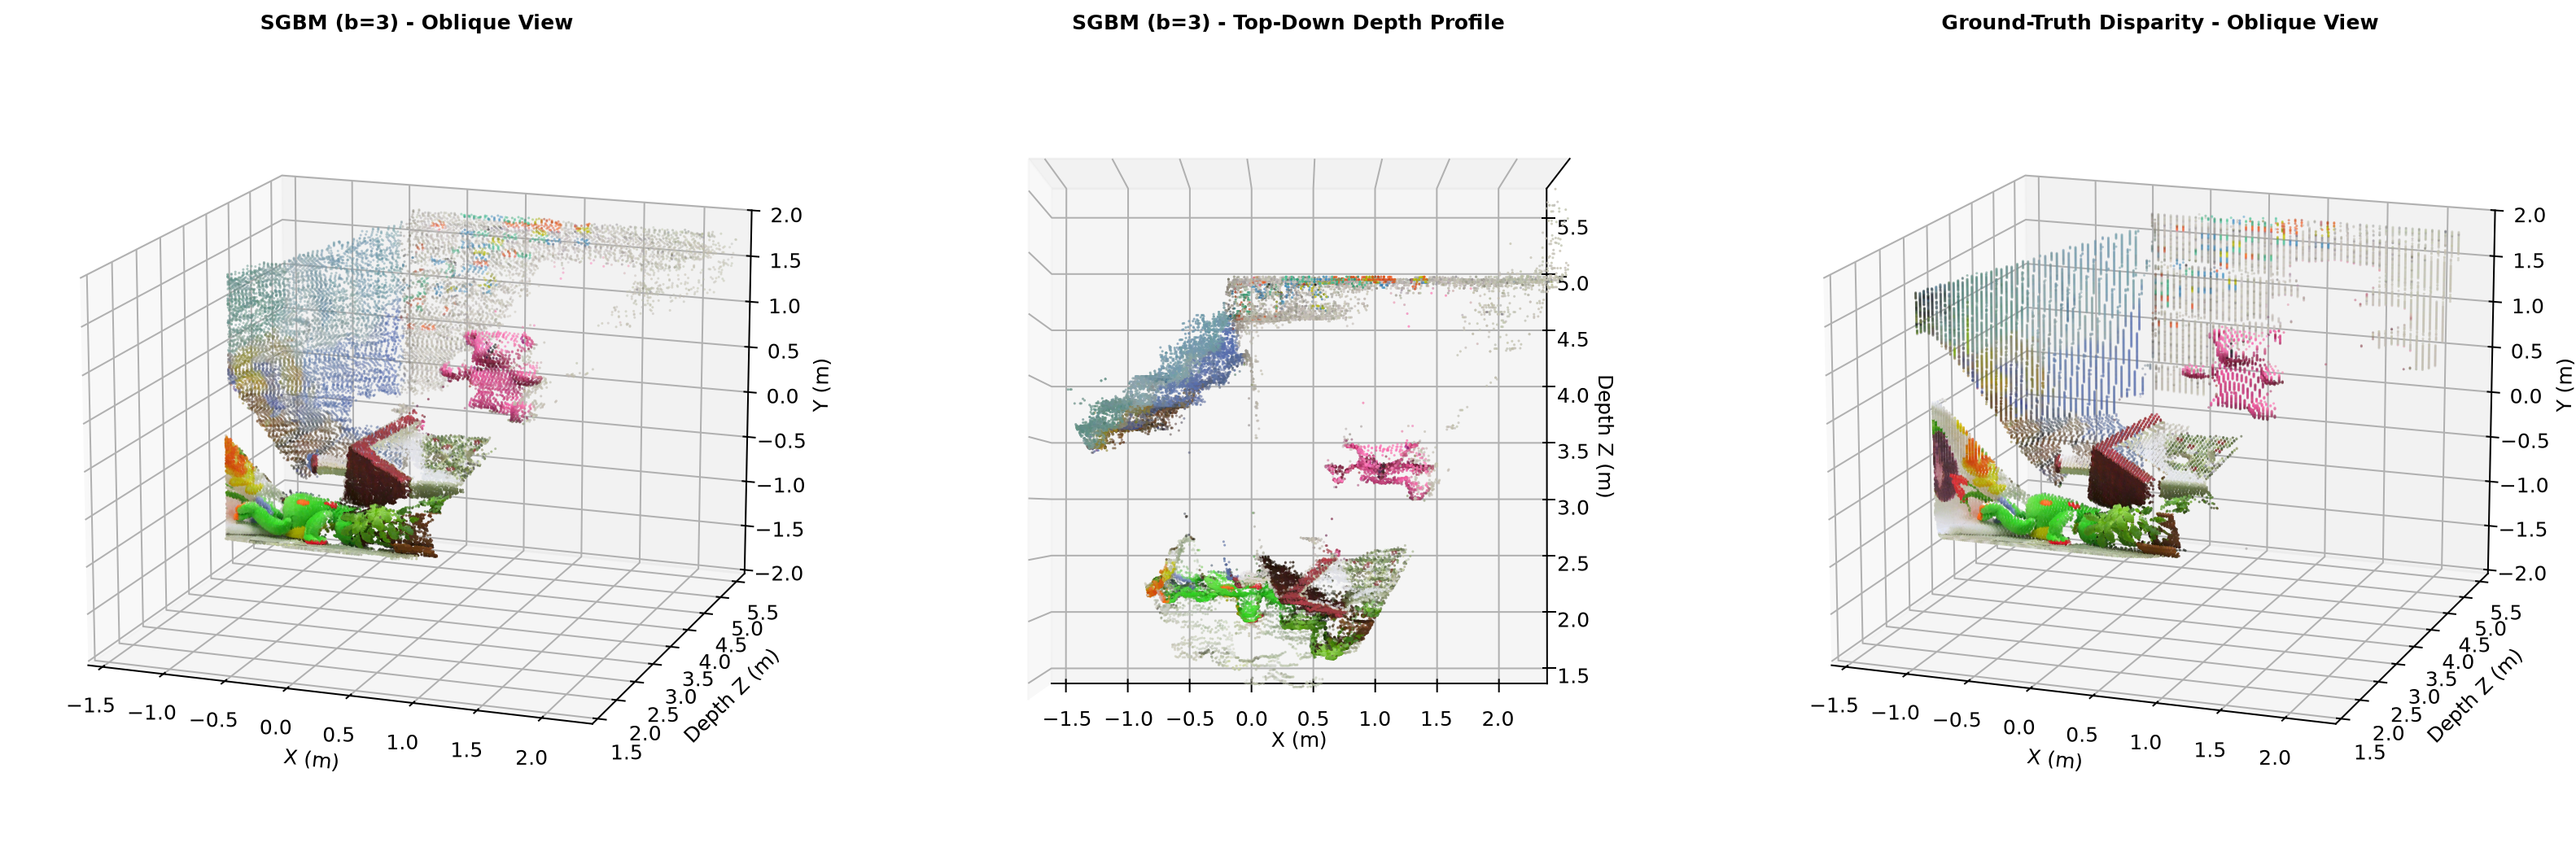
\includegraphics[width=\textwidth]{figures/point_cloud_views.png}
    \caption{Part B: 3D point cloud from SGBM ($b=3$, $d=64$) in oblique and top-down views, next to the point cloud obtained from the ground-truth disparity.}
    \label{fig:pointcloud}
\end{figure}

\subsection{Comparative Analysis}
Table \ref{tab:part_b} summarizes the quantitative metrics across BM and SGBM parameter configurations. The epipolar errors ($0.2389$ px symmetric, $0.1689$ px Sampson) are shared by all rows because $\mathbf{F}$ is estimated once from sparse SIFT matches.

\begin{table}[H]
\centering
\caption{Quantitative comparison between BM and SGBM on Teddy (accuracy measured on non-occluded pixels).}
\label{tab:part_b}
\footnotesize
\resizebox{\textwidth}{!}{%
\begin{tabular}{lcccccccc}
\toprule
\textbf{Method} & \textbf{blockSize} & \textbf{numDisp} & \textbf{Valid (\%)} $\uparrow$ & \textbf{Valid Non-occ. (\%)} $\uparrow$ & \textbf{RMSE (px)} $\downarrow$ & \textbf{Bad $>$1px (\%)} $\downarrow$ & \textbf{Bad $>$2px (\%)} $\downarrow$ & \textbf{Time (ms)} $\downarrow$ \\
\midrule
BM & 9 & 64 & 68.59 & 75.34 & \textbf{1.745} & \textbf{5.16} & 4.29 & 4.34 \\
BM & 15 & 64 & 70.54 & 76.80 & 1.874 & 7.39 & 6.02 & 4.43 \\
BM & 21 & 64 & 69.66 & 75.72 & 1.974 & 8.71 & 7.07 & \textbf{4.05} \\
SGBM & 3 & 64 & \textbf{81.12} & \textbf{88.21} & 2.092 & 6.35 & \textbf{3.43} & 10.42 \\
SGBM & 5 & 64 & 80.70 & 87.73 & 2.833 & 7.04 & 4.08 & 9.86 \\
SGBM & 9 & 64 & 80.88 & 87.79 & 3.071 & 9.16 & 5.81 & 8.59 \\
SGBM & 5 & 96 & 73.77 & 79.86 & 3.009 & 7.40 & 4.28 & 9.39 \\
\bottomrule
\end{tabular}}
\end{table}

\textbf{Qualitative Discussion:}
\begin{itemize}
    \item \textbf{Coverage \& Smoothness:} SGBM recovers $81\%$ of all pixels ($88\%$ of non-occluded pixels) versus about $70\%$ for BM. BM leaves holes on weakly textured surfaces such as the white roof of the wooden house, the smooth painting in the upper left and the plain wall behind the teddy bear, where the SAD cost has no clear minimum and the uniqueness test rejects the match. SGBM fills these regions by propagating disparities along its 1D paths, producing piecewise-smooth surfaces.
    \item \textbf{Accuracy Trade-off:} SGBM $b=3$ has the lowest Bad$>$2px rate ($3.43\%$) while also being the densest. BM keeps a slightly lower RMSE and Bad$>$1px because it only outputs confident matches; the extra pixels SGBM fills include a few gross errors (e.g., the strongly slanted newspaper on the floor) that dominate the squared error.
    \item \textbf{Block Size:} Larger windows hurt both methods on Teddy. For BM, growing $b$ from $9$ to $21$ removes speckle noise on the textured poster but raises Bad$>$2px from $4.29\%$ to $7.07\%$ through \emph{foreground fattening}: object silhouettes (teddy bear, house edge, plant leaves) bleed into the background. SGBM degrades similarly from $3.43\%$ ($b=3$) to $5.81\%$ ($b=9$) as thin leaves and the thin post under the house are smoothed away.
    \item \textbf{Disparity Range:} Since the true disparity never exceeds $53$ px, \texttt{numDisparities} $=64$ is sufficient. Increasing it to $96$ brings no accuracy gain and widens the invalid band on the left border (the first $d$ columns cannot be matched), lowering coverage from $80.70\%$ to $73.77\%$.
    \item \textbf{Occlusions \& Boundaries:} Both methods correctly mark most occluded pixels (left of the house, the gap behind the frog, between the leaves) as invalid, aided by the uniqueness and left-right checks (Figure \ref{fig:errormaps}). Remaining errors concentrate along depth discontinuities and in the fine plant structure.
    \item \textbf{Runtime:} BM runs in about $4$--$4.4$ ms, roughly $2$--$2.5\times$ faster than SGBM ($8.6$--$10.4$ ms) at this $450\times 375$ resolution.
    \item \textbf{3D Geometry:} The SGBM point cloud (Figure \ref{fig:pointcloud}) reproduces the depth layering of the ground-truth cloud: the frog and potted plants in front ($Z \approx 1.5$--$2.5$ m), the wooden house and teddy bear in the middle, and the poster wall in the back ($Z \approx 5$ m). The top-down view shows the slanted painting plane on the left and the flat back wall. Residual outliers appear as thin streaks at object boundaries, which correspond to the red error pixels in Figure \ref{fig:errormaps}.
\end{itemize}

\section{Part C: Image Stitching}
\subsection{Methodology}
Four overlapping views $\{I_1, I_2, I_3, I_4\}$ with $50\%$ horizontal overlap and perspective perturbations are extracted from the reference scene (Figure \ref{fig:input_views}). We compare three feature detectors/descriptors: \textbf{SIFT} (float DoG + gradient histogram, $\ell_2$ norm), \textbf{ORB} (FAST + oriented BRIEF binary descriptor, Hamming norm), and \textbf{AKAZE} (non-linear diffusion scale space). Candidate 2-NN matches passing Lowe's ratio test ($d_1 < 0.75 d_2$) are used to estimate $3\times 3$ planar homographies $\mathbf{H}$ via RANSAC ($\tau \in \{2.0, 4.0\}\text{ px}$). Using View 2 as the central anchor, chained homographies $\mathbf{H}_{4\to 2} = \mathbf{H}_{3\to 2}\mathbf{H}_{4\to 3}$ warp all views onto a common canvas, blended via Euclidean distance-transform feathering weights $w_k(x,y) = d_k(x,y) / \sum_j d_j(x,y)$.

\subsection{Implementation and Results}
Figure \ref{fig:input_views} shows the four input views, and Figure \ref{fig:stitching_comp} presents the RANSAC inlier correspondences alongside the final 4-view stitched panoramas for SIFT, ORB, and AKAZE.

\begin{figure}[H]
    \centering
    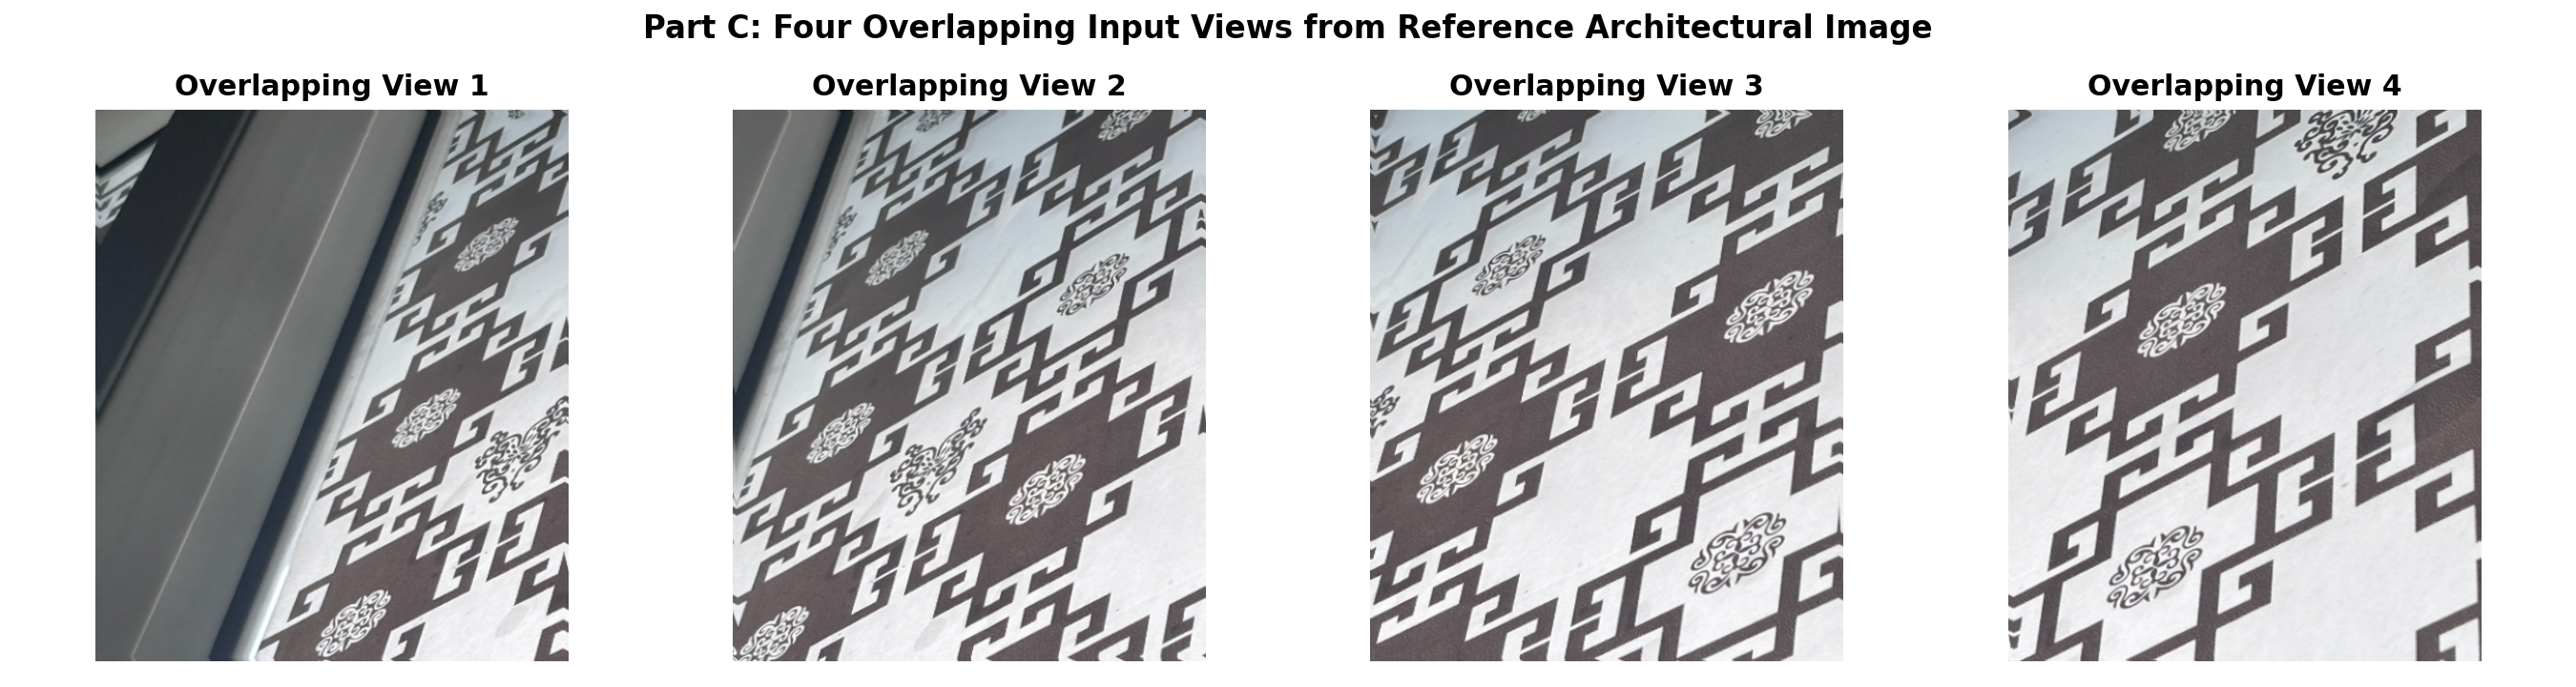
\includegraphics[width=0.95\textwidth]{figures/input_4_views.png}
    \caption{Part C: Four overlapping perspective input views generated from the reference image.}
    \label{fig:input_views}
\end{figure}

\begin{figure}[H]
    \centering
    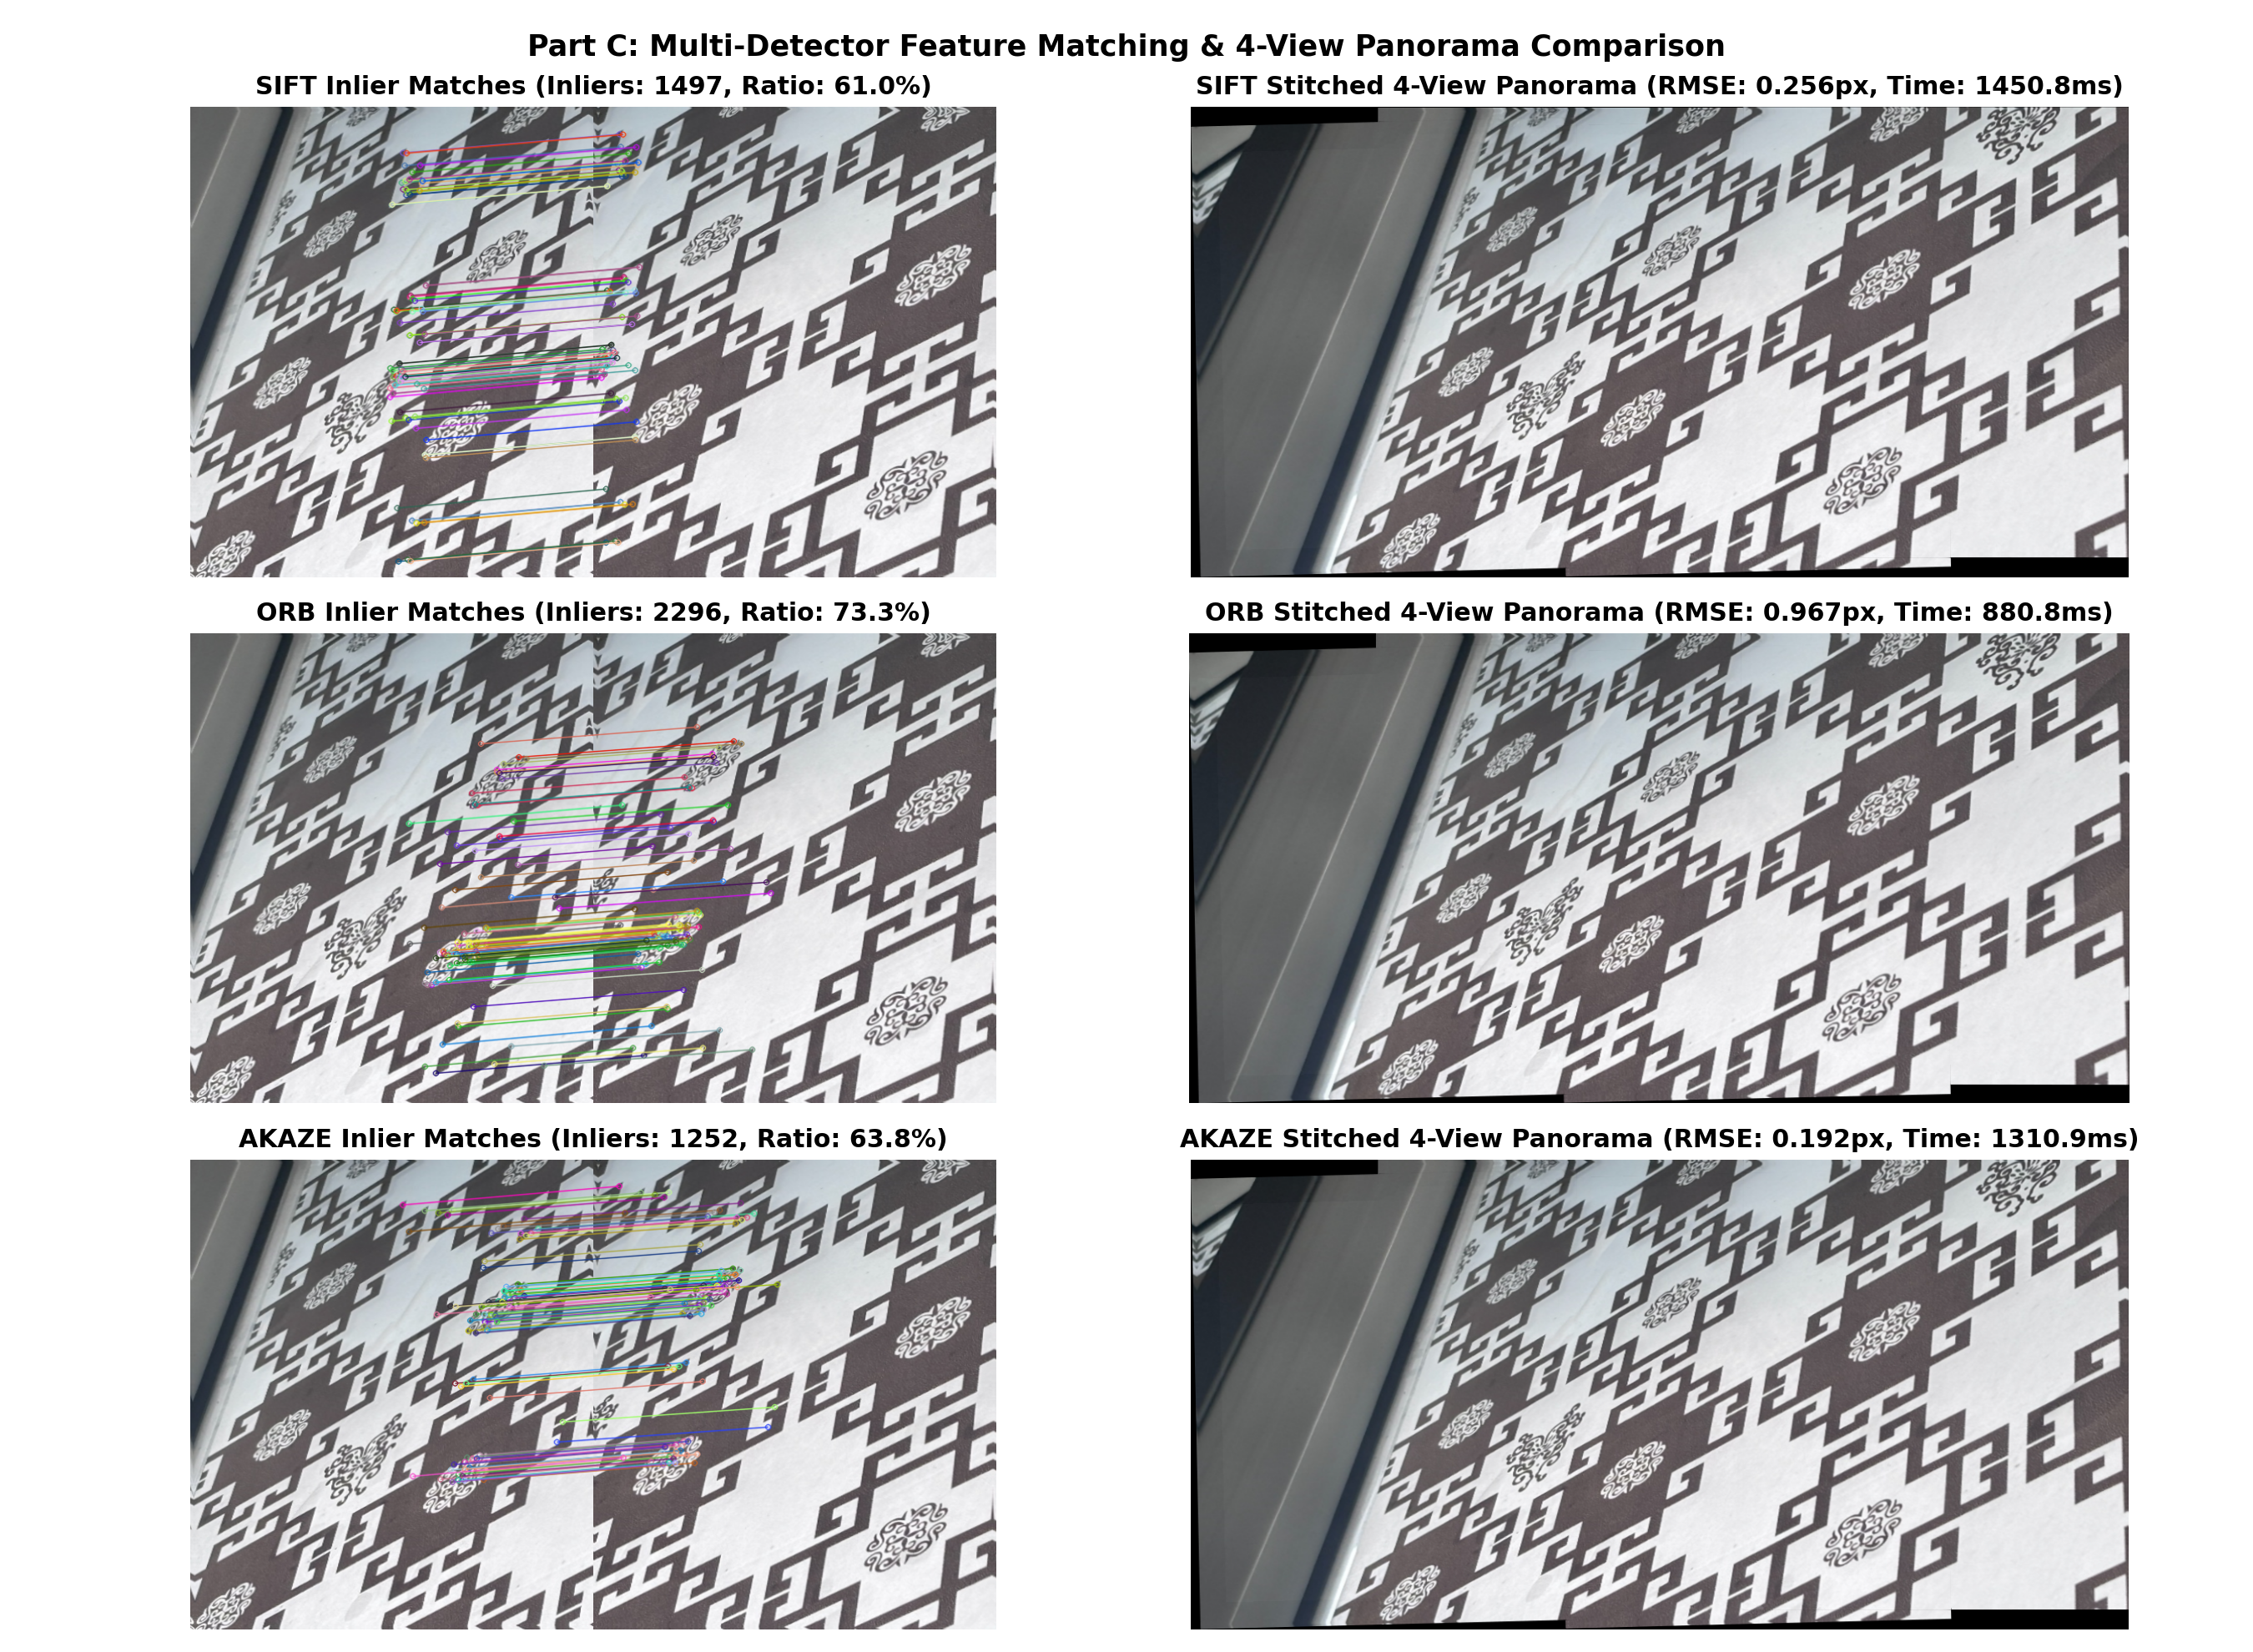
\includegraphics[width=0.96\textwidth]{figures/stitching_comparison.png}
    \caption{Part C: Inlier feature matches (left) and final 4-view stitched panoramas (right) for SIFT, ORB, and AKAZE.}
    \label{fig:stitching_comp}
\end{figure}

\subsection{Comparative Analysis}
Table \ref{tab:part_c} summarizes the quantitative metrics across detectors and RANSAC thresholds.

\begin{table}[H]
\centering
\caption{Quantitative comparison of SIFT, ORB, and AKAZE for 4-view panoramic stitching.}
\label{tab:part_c}
\footnotesize
\begin{tabular}{lccccccc}
\toprule
\textbf{Detector} & \textbf{RANSAC $\tau$} & \textbf{Keypoints} & \textbf{Init Matches} & \textbf{Inliers} & \textbf{Inlier Ratio (\%)} $\uparrow$ & \textbf{RMSE (px)} $\downarrow$ & \textbf{Time (ms)} $\downarrow$ \\
\midrule
SIFT & 2.0 px & 10,043 & 2,449 & 1,488 & 60.58\% & 0.207 & 1606.60 \\
SIFT & 4.0 px & 10,043 & 2,449 & 1,497 & 60.95\% & 0.256 & 1450.76 \\
ORB & 2.0 px & \textbf{17,582} & \textbf{3,113} & 1,977 & 62.66\% & 0.817 & \textbf{856.84} \\
ORB & 4.0 px & \textbf{17,582} & \textbf{3,113} & \textbf{2,296} & \textbf{73.29\%} & 0.967 & 880.76 \\
AKAZE & 4.0 px & 7,285 & 1,951 & 1,252 & 63.84\% & \textbf{0.192} & 1310.94 \\
\bottomrule
\end{tabular}
\end{table}

\textbf{Qualitative Discussion:}
\begin{itemize}
    \item \textbf{Geometric Alignment \& Reprojection Error:} \textbf{AKAZE} ($\text{RMSE}=0.192\text{ px}$) and \textbf{SIFT} ($\text{RMSE}=0.207\text{ px}$) achieve $4\times$ lower reprojection error than \textbf{ORB} ($\text{RMSE}=0.967\text{ px}$) due to continuous sub-pixel keypoint localization. Notice that repetitive geometric fretwork patterns cause around $36\%$--$39\%$ ambiguous initial matches, which are effectively rejected by RANSAC.
    \item \textbf{Computational Efficiency:} \textbf{ORB} is the fastest pipeline ($856.84\text{ ms}$) and detects the largest number of keypoints ($17,582$) and inliers ($2,296$) concentrated along high-contrast corners.
    \item \textbf{Seam Visibility \& Blending:} Distance-transform feather blending completely eliminates visible seams and ghosting artifacts across all four overlapping views, preserving continuous diagonal fretwork lines across the entire panorama.
\end{itemize}

\section{Conclusion}
This project systematically evaluated classical computer vision pipelines for image filtering, 3D stereo reconstruction, and panoramic stitching. Key takeaways include: (1) non-linear Median filtering ($3\times 3$) is indispensable for impulsive noise while $3\times 3$ Gaussian filtering best preserves high-frequency textures under Gaussian noise; (2) on Teddy, SGBM with a small window ($b=3$) gives both the densest ($81.12\%$ valid) and most accurate ($3.43\%$ bad pixels) disparity map, while larger windows cause foreground fattening for both BM and SGBM; and (3) SIFT and AKAZE provide superior sub-pixel homography alignment compared to faster binary ORB descriptors. Future work includes integrating Weighted Least Squares (WLS) disparity post-filtering and Multi-Band Laplacian Pyramid blending.

\begin{thebibliography}{9}
\bibitem{szeliski} R. Szeliski, \textit{Computer Vision: Algorithms and Applications}, 2nd ed. Springer, 2022.
\bibitem{lowe} D. G. Lowe, ``Distinctive image features from scale-invariant keypoints,'' \textit{IJCV}, vol. 60, no. 2, pp. 91--110, 2004.
\bibitem{hirschmuller} H. Hirschmuller, ``Stereo processing by semiglobal matching and mutual information,'' \textit{IEEE TPAMI}, vol. 30, no. 2, pp. 328--341, 2008.
\bibitem{middlebury} D. Scharstein and R. Szeliski, ``High-accuracy stereo depth maps using structured light,'' in \textit{Proc. IEEE CVPR}, 2003, pp. 195--202.
\bibitem{rublee} E. Rublee, V. Rabaud, K. Konolige, and G. Bradski, ``ORB: An efficient alternative to SIFT or SURF,'' in \textit{Proc. IEEE ICCV}, 2011, pp. 2564--2571.
\end{thebibliography}

\appendix
\section{Appendix: Python Source Code}
The complete Python scripts (\texttt{part\_a\_filtering.py}, \texttt{part\_b\_stereo\_3d.py}, and \texttt{part\_c\_stitching.py}) are included in the submission archive and summarized below.
\lstinputlisting[caption={Part A: Image Filtering and Enhancement (\texttt{part\_a\_filtering.py})}]{../part_a_filtering.py}
\lstinputlisting[caption={Part B: 3D Stereo Reconstruction (\texttt{part\_b\_stereo\_3d.py})}]{../part_b_stereo_3d.py}
\lstinputlisting[caption={Part C: 4-View Image Stitching (\texttt{part\_c\_stitching.py})}]{../part_c_stitching.py}

\end{document}
